\section{Definition}\label{sec:definition}

\begin{wrapfigure}{R}{0.3\textwidth}
\centering
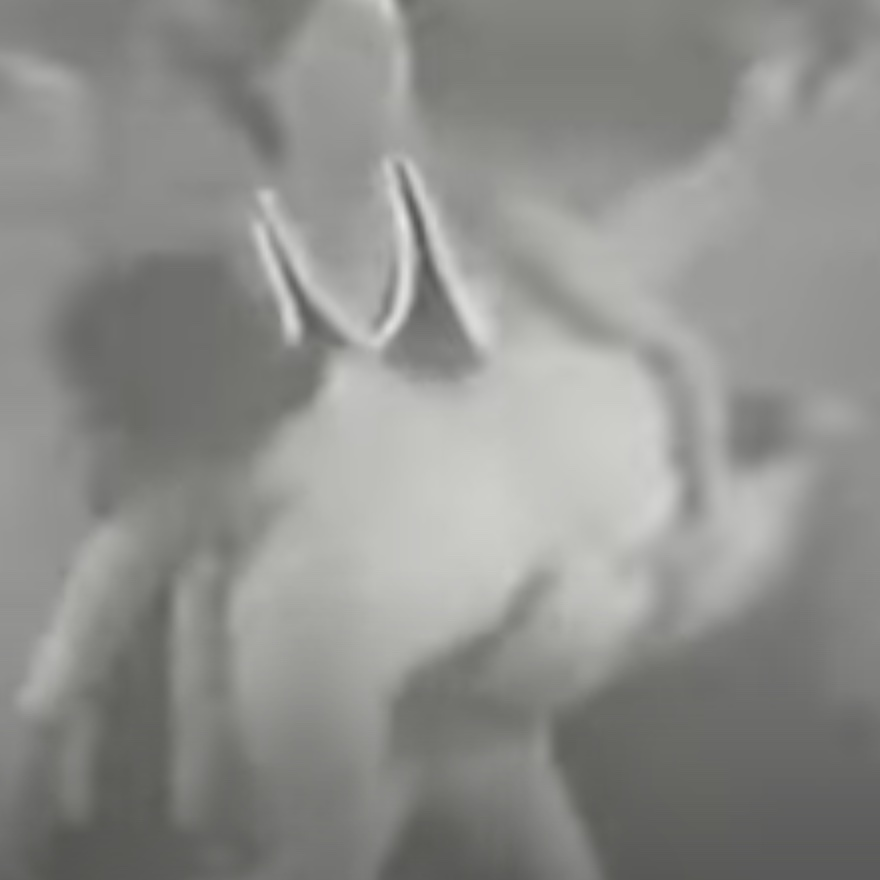
\includegraphics[width=0.25\textwidth]{images/definition}
\end{wrapfigure}

So what is CI? A dance, a sport, an (visceral) art-form or art-sport, partner acrobatics or martial arts?
Well, maybe all of it, or maybe depending on how one approaches it and what one's background is and where the emphasis is put on.
Let's have a look at the different views on it, and by also looking at its history it might get more clear what it is, or what it can be for you.

Emphasize is put on:
\begin{itemize}
	\item \textbf{Experimental dance}: practice-based research in dance laboratories
	\item \textbf{Theatrical form}: improvised performances and lectures-demonstrations
	\item \textbf{Educational tool}: training for professional dancers in improvisation
	\item \textbf{Awareness practice}: being able to listen to the subtleties in contact
	\item \textbf{Social dancing}: at informal gatherings called ``jams''
\end{itemize}

At its core it involves mindfulness, sensing and collecting information which requires full presence and attention.
And yes, it is even related to other improvisation practices like improvisation acting: the ``Yes, and \ldots'' concept expressed physically.

This art form is not only for the young and well-trained, as there is no real requirement for acrobatic performance.
The body just needs to be mobile and the bones bear some weight.

\subsection{Dance}\label{subsec:dance}

It could be considered a form of improvised partner dancing, embedded in contemporary and (post-)modern dance form.
Dance improvisation existed already before CI, but it didn't have the contact aspect as CI has, most of all the shared point of contact.
The development in dance history goes like from ballet, to modern (Martha Gram, John Cage, Cunningham), to contemporary (improvisation became not only a research tool, but a performance itself).
They are mostly vertically, meaning standing and there is no floorwork.
In CI we roll over each other on the floor, something which would be seen as rather unusual in other styles.
CI uses a three-dimensional spherical space, were every body-part can be a foot (pushed against the ground).

CI is an improvised ``art-form'' (or ``art-sport''), thus without any predefined choreography.
Sometimes CI is used in choreographies, which is then called ``partnering''.
CI is an exploration, a way to try to ``break the system'' as it is improvised.
Nevertheless, CI is not a thing in the professional dance world, a world where they are walking with very ``nice'' movements.

It is not so much that as a CI dancer you are serving the audience (in a performance), but rather that the audience is joining you.
It's about getting a visceral reaction from the audience of an improvisation art-form, that they want to join.
Ultimately there is no difference between dancers and the audience, no hierarchy exists.

It is distinct from other partner dance styles, as those are more focused on the social aspect, whereas CI comes from the art world.
Others are also very much gender-roled, where usually the man would lead, and the woman would follow (exceptions exist like for example Lindy Hop).
In CI, everyone dances with everyone, without any clearly defined role.

CI has a strong focus on the physical aspect: How to survive a high impact volume, which leads to either to crash or to fall.
Lindy Hop is for example also very strong in acrobatics, which Zouk also does a little.
Thinking about taking/lifting people on your body, on your core/center.

There is also a difference in styling, as many aesthetically pleasing dance styles would ``dress to impress''.
In CI, we would typically come wearing our pyjamas, sloppy, cosy, comfy, pragmatic.

\subsection{Martial Art}\label{subsec:martial-art}

It is also combined with some minor aspects of eastern philosophy and a few things from the 1960s hippie culture.
Reason being that some founders of CI had their background in the Japanese martial art of Aikido, which is similar to (Brazilian Jiu Jitsu), to gently receive incoming force and deflect it in circular movements.

\subsection{Applied Physics}\label{subsec:applied-physics}

An exploration of physical forces of one's body in relationship to others by using principles of sharing weight, touch, and movement awareness, while moving in contact and the ground.
To play with the artistry of falling off balance and counterbalance, with gravity and physics.
To learn the mechanics of the body to handle someone's weight or to be lifted, along with breathing techniques.
Alternatively: A three-body-problem with two dancers, being shaped/moved by momentum, gravity, and force, dealing with the third body, the ground/earth.

\subsection{Acrobatics}\label{subsec:acrobatics}

The main founder, Steve Paxton himself was a gymnast, and that might be the reason why still some styles resemble more partner acrobatics than dancing.
The many (demanding) lifts, and the high velocity and high impact movements can require a high level of fitness of the practitioners.

\subsection{Community}\label{subsec:community}

The founders decided to keep CI open to a broad community, thus it has never been institutionalised, neither is the name copyright protected.
Yet, [Contact Quarterly](https://contactquarterly.com) and [ECITE](http://www.ecite.org) can be considered the two main international forums ensuring the quality and continuity of CI.

There is a broad global community, which organizes social dances, so-called ``jams'', and practitioners often overlap with the Ecstatic Dance communities.

Speaking of Ecstatic Dance: Many people from that background often claim to have done ``contact'' yet actually have no idea about CI.
This confusion is about ``touch based partner dance'' and the art-form of CI.
These people might also bring in a slight different (sensual-sexual, maybe Tantric) attitude which is not welcome in CI.

\subsection{Jams}\label{subsec:jams}

Jams, as stated already above, are social gatherings without any leader; similar to jazz jam sessions or milongas in tango.
It's an opportunity to practice freely, where people can meet and negotiate together their dance or observe the practice of their partners.
Occasions to meet other fellow practitioners, friends or strangers, old, young, experienced, novice.
It's a hybrid between bodily meditation, psycho-kinesthetic therapy, sports training and a dance improvised session.
They can be regularly in a studio for a few hours, or longer retreat jams for several days in spring resorts where it can be practiced at any hour of the day.

\subsection{Historically}\label{subsec:historically}

In the early beginnings (1970s) every time they practiced it, they would redefine it, asking the same question over and over again: What is CI \textit{now}?

An early definition by Steve Paxton and others (CQ Vol. 5:1, Fall 1979):

A continuously evolving system of improvised movement.
Two bodies, communicating with each other in physical contact, creating a relationship with the physical laws (motion, gravity, momentum, inertia).
Sensitive, thus relaxed of unnecessary muscular tension, and willing to experience a natural flow.
Techniques may include: Rolling, falling, being upside down, following, supporting and giving weight.

A physical dialogue ranging from stillness to highly energetic exchange.
Alert enough to stay in an energetic state of physical disorientation, trusting your survival instincts.
A free play seeking for balanced movements, leading to a physical and emotional truth, shared at the moment, leaving you informed, centered, and enlivened

\subsection{Definitions}\label{subsec:definitions}

Definitions, and the same with any terminology, are time-, space- and person-dependent.
Just as with the improvised nature of CI, it is a constantly moving target.
By asking the same question a week later, the answer one receives will already be different.

Yet, there is a rough body of agreement (a congruent understanding) of what it is, and what it is not, leading to a definition stable across time, space, and practitioner.
It's like a tree: The trunk (the agreed principles) and it's branches and leaves (the styles, adaptations), representing the edges where one can play freely.

\textbf{Steve Paxton} himself stated in 1979: \textit{The exigencies of the form dictate a mode of movement which is relaxed, constantly aware and prepared, and onflowing. As a basic focus, the dancers remain in physical touch, mutually supportive and innovative, meditating upon the physical laws relating to their masses: gravity, momentum, inertia, and friction. They do not strive to achieve results, but rather, to meet the constantly changing physical reality with appropriate placement and energy.}

\textbf{Nancy Start Smith} once mentioned, it ``\textit{resembles other familiar duet forms, such as the embrace, wrestling, surfing, martial arts, and the Jitterbug (Lindy Hop and swing dances), encompassing a wide range of movement from stillness to highly athletic}''.

\textbf{Daniel Lepkoff} states about the core of CI, to ``\textit{put focus on bodily awareness and physical reflexes, rather than consciously controlled movements. Precedence of body experience first, and mindful cognition second, is an essential distinction between CI and other approaches to dance.}''

\textbf{Ray Chung} once announced in an workshop 2009 that CI is ``\textit{an open-ended exploration of the kinaesthetic possibilities of bodies moving through contact. Sometimes wild and athletic, sometimes quiet and meditative, it is a form open to all bodies and enquiring minds.}''

\subsection{Beyond CI}\label{subsec:beyond-ci}

CI is for sure not a pure \textbf{martial art}, as it has no claim to have any real fighting application.
Nor is it a competitive \textbf{sport} in any way, as there are no competitions and due to it's artistic nature it would be difficult (impossible?) to judge one as being better than the other.
It has many aspects of partner \textbf{acrobatics}, but lacks many possibilities due to its confining principles (e.g.\ grabbing/manipulation).

It is also not really your regular \textbf{dance} form like salsa or tango, due to several reasons: We don't dress to impress but rather show up with our pyjamas; we don't even necessarily dance in order to look good or aesthetically; we focus more on the internal and interpersonal aspects than external ones; we dance often without music; there are no real techniques which can be learned but only guiding principles from which some specific movements can emerge; and so forth.

As it is the case with so many (all?) disciplines, once the rule has been understood, it can be broken by the student, thus \textbf{becoming a master} of it.
Furthermore, a system is supposed to be of service to the user, and its boundaries and dogma should not limit but enrich the applicant.
Whenever the purpose is hindered by the system, the system shall be left behind and we should remember the original goal which was there in the first place, and not to serve the gods we created.
